% Path: docs/report_final_en.tex
\documentclass[11pt,a4paper]{article}

\usepackage[utf8]{inputenc}
\usepackage[T1]{fontenc}
\usepackage[english]{babel}
\usepackage{geometry}
\usepackage{booktabs}
\usepackage{graphicx}
\usepackage{float}
\usepackage{hyperref}
\usepackage{enumitem}
\usepackage{setspace}

\geometry{margin=1in}
\onehalfspacing

\title{Image\_Captioning\_CNN\_LSTM}
\author{Giuseppe Dimonte \\ Student ID 367431}
\date{Academic Year 2025/26}

\begin{document}

\begin{titlepage}
\centering
{\Large University of Parma \par}
\vspace{0.3cm}
{\large Department of Engineering and Architecture \par}
\vspace{0.3cm}
{\large Degree Program in Computer Engineering \par}
{\large Curriculum: Artificial Intelligence \par}
\vspace{1.2cm}
{\Large \textbf{Deep Learning and Generative Models} \par}
\vspace{0.5cm}
{\large Instructor: Prof. Andrea Prati \par}
\vspace{1.5cm}
{\huge \textbf{Image\_Captioning\_CNN\_LSTM} \par}
\vspace{1.5cm}
{\large \textbf{Student:} Giuseppe Dimonte \par}
{\large \textbf{Student ID:} 367431 \par}
{\large \textbf{Email:} giuseppe.dimonte@studenti.unipr.it \par}
\vfill
{\large Academic Year 2025/26 \par}
\end{titlepage}

\tableofcontents
\newpage

\begin{abstract}
This report presents the implementation and evaluation of a CNN-LSTM image captioning system trained on Flickr8k. The project covers the complete pipeline required by the assignment: caption preprocessing, vocabulary construction, training/validation file preparation, supervised training, BLEU-based evaluation, and qualitative analysis. A controlled experimental comparison was conducted on four configurations: baseline, removal of scheduled sampling, removal of label smoothing, and CNN fine-tuning. The best result was obtained by the fine-tuning configuration, which achieved BLEU-4 equal to 0.0649, outperforming the baseline BLEU-4 score of 0.0472.
\end{abstract}

\section{Introduction}

Image captioning is a multimodal problem in which a system receives an image and must produce a natural language description of its content. The task combines visual recognition and language generation, and can therefore be naturally formulated as an image-to-sequence problem.

The objective of this project was to implement a complete CNN-LSTM captioning pipeline in accordance with the course assignment. Beyond the model itself, the work also focused on making the entire workflow reproducible, from data preparation to systematic experimental comparison.

\section{Assignment Requirements}

The assignment required:
\begin{itemize}[leftmargin=*]
    \item the use of Flickr8k;
    \item a CNN-LSTM architecture;
    \item caption cleaning;
    \item vocabulary construction and export;
    \item pairing image features with tokenized captions during training;
    \item word prediction through the decoder output during testing.
\end{itemize}

The final repository satisfies these requirements through a modular and reproducible implementation.

\section{Dataset and Preprocessing}

\subsection{Flickr8k}

Flickr8k associates each image with five reference captions. In the final project, the dataset was transformed into reproducible artifacts:
\begin{itemize}[leftmargin=*]
    \item \texttt{data/vocab.json}
    \item \texttt{data/Flickr8k\_text/train.csv}
    \item \texttt{data/Flickr8k\_text/val.csv}
    \item \texttt{data/Flickr8k\_text/test\_captions.json}
\end{itemize}

Final observed sizes:
\begin{itemize}[leftmargin=*]
    \item 30000 training caption rows
    \item 5000 validation caption rows
    \item 1000 test images
    \item 5 reference captions per image
\end{itemize}

\subsection{Caption Cleaning}

Captions were preprocessed using:
\begin{itemize}[leftmargin=*]
    \item lowercase conversion
    \item punctuation removal
    \item digit removal
    \item single-letter word removal
    \item whitespace normalization
\end{itemize}

The final vocabulary contains 2985 tokens, including the special tokens \texttt{<pad>}, \texttt{<bos>}, \texttt{<eos>}, and \texttt{<unk>}.

\section{Model Architecture}

The system follows an encoder-decoder design.

\subsection{Encoder}

The encoder uses pretrained InceptionV3. The classification head is removed and the extracted features are projected into the decoder embedding space.

\subsection{Decoder}

The decoder is a single-layer LSTM. During training, it receives the image-conditioned representation together with the tokenized caption. A final linear layer maps hidden states to vocabulary logits for next-token prediction.

\subsection{Training Features}

The implemented training loop supports:
\begin{itemize}[leftmargin=*]
    \item scheduled sampling
    \item label smoothing
    \item gradient clipping
    \item checkpoint saving
    \item checkpoint resume
    \item BLEU-1, BLEU-2, BLEU-3, BLEU-4 evaluation
\end{itemize}

\section{Implementation Details}

The final repository is organized as follows:
\begin{itemize}[leftmargin=*]
    \item \texttt{src/vocab\_builder.py}: cleaning, vocabulary construction, split export
    \item \texttt{src/prepare\_data.py}: convenience data preparation script
    \item \texttt{src/dataset.py}: dataset loading and batching
    \item \texttt{src/model.py}: CNN-LSTM definition
    \item \texttt{src/train.py}: training loop and checkpoint logic
    \item \texttt{src/eval.py}: caption generation and BLEU evaluation
    \item \texttt{src/visualize.py}: qualitative visualization
    \item \texttt{src/ui\_streamlit.py}: optional interactive interface
\end{itemize}

During revision, several structural issues were corrected, including:
\begin{itemize}[leftmargin=*]
    \item incorrect parsing of Flickr8k captions
    \item missing train/validation/test artifacts
    \item incorrect next-token loss alignment
    \item ineffective encoder fine-tuning
\end{itemize}

\section{Experimental Setup}

All final experiments were executed in the \texttt{captioning} environment with PyTorch \texttt{2.9.1+cpu}. The device used for training and evaluation was CPU.

Compared configurations:
\begin{enumerate}[leftmargin=*]
    \item Baseline
    \item No Scheduled Sampling
    \item No Label Smoothing
    \item Fine-tuning
\end{enumerate}

All final runs were executed for 5 epochs.

\section{Quantitative Results}

\begin{table}[H]
\centering
\caption{BLEU comparison across the final experiments.}
\begin{tabular}{lcccc}
\toprule
Experiment & BLEU-1 & BLEU-2 & BLEU-3 & BLEU-4 \\
\midrule
Baseline & 0.2553 & 0.1556 & 0.0928 & 0.0472 \\
No Scheduled Sampling & 0.2232 & 0.1242 & 0.0717 & 0.0396 \\
No Label Smoothing & 0.2404 & 0.1435 & 0.0809 & 0.0394 \\
Fine-tuning & 0.3301 & 0.2022 & 0.1189 & 0.0649 \\
\bottomrule
\end{tabular}
\end{table}

\begin{table}[H]
\centering
\caption{Training summary.}
\begin{tabular}{lccc}
\toprule
Experiment & Best Val Loss & Final Train Loss & Final Val Loss \\
\midrule
Baseline & 4.1927 & 4.8016 & 4.2332 \\
No Scheduled Sampling & 4.0106 & 3.5373 & 4.0234 \\
No Label Smoothing & 3.5029 & 4.0860 & 3.5738 \\
Fine-tuning & 3.6614 & 4.7512 & 4.2861 \\
\bottomrule
\end{tabular}
\end{table}

\section{Discussion}

The baseline provides the reference point for comparison. Removing scheduled sampling lowers all BLEU metrics, showing that scheduled sampling improves generalization during autoregressive caption generation.

Removing label smoothing also reduces BLEU performance, indicating that label smoothing contributes positively in this setup.

The best overall result is achieved by the fine-tuning configuration. The BLEU-4 score increases from 0.0472 in the baseline to 0.0649 with fine-tuning, making it the strongest final configuration in this study.

\section{Qualitative Analysis}

\begin{figure}[H]
    \centering
    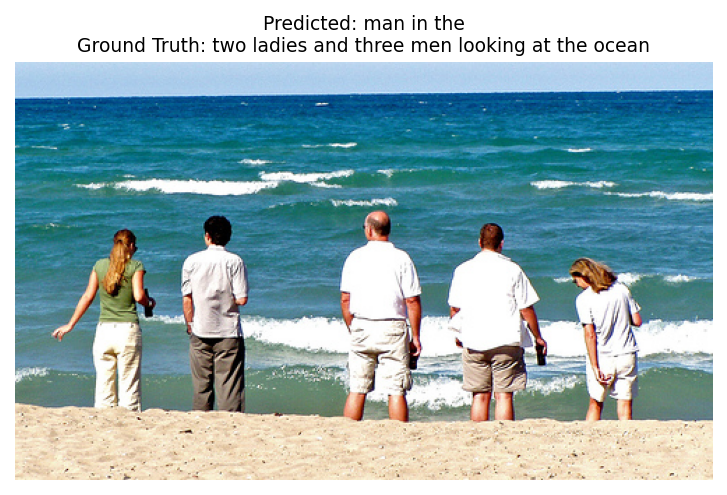
\includegraphics[width=0.8\textwidth]{selected_figures/baseline_example.png}
    \caption{Representative baseline output. The prediction is partially related to the scene but remains generic and incomplete relative to the reference caption.}
    \label{fig:baseline_en}
\end{figure}

\begin{figure}[H]
    \centering
    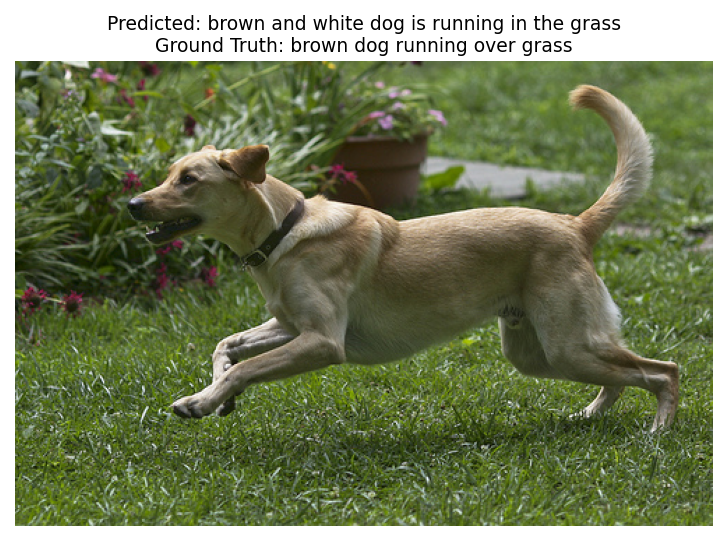
\includegraphics[width=0.8\textwidth]{selected_figures/finetune_example.png}
    \caption{Representative fine-tuned output. The generated caption correctly identifies the main object and action.}
    \label{fig:finetune_en}
\end{figure}

\begin{figure}[H]
    \centering
    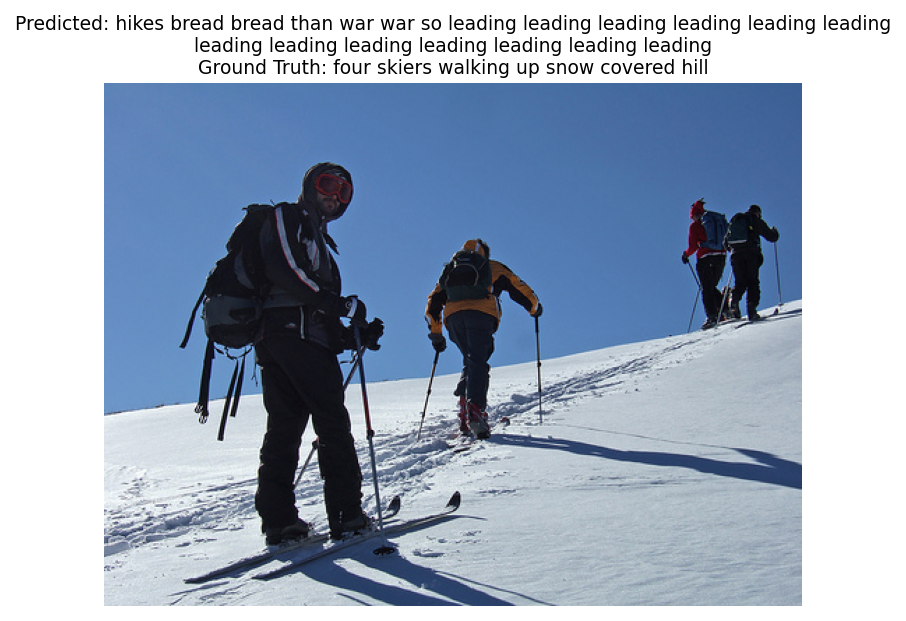
\includegraphics[width=0.8\textwidth]{selected_figures/failure_case.png}
    \caption{Failure case. The output is repetitive and semantically unstable, illustrating an important residual limitation of the model.}
    \label{fig:failure_en}
\end{figure}

\section{Limitations}

\begin{itemize}[leftmargin=*]
    \item All experiments were executed on CPU, resulting in long training times.
    \item Flickr8k is relatively small for image captioning.
    \item The work focuses on a classical CNN-LSTM architecture and does not compare with transformer-based alternatives.
\end{itemize}

\section{Conclusion}

This project implemented a complete CNN-LSTM image captioning pipeline on Flickr8k, covering preprocessing, vocabulary generation, supervised training, evaluation, and qualitative analysis. The final experiments show that scheduled sampling and label smoothing both improve performance relative to their corresponding ablations, while CNN fine-tuning provides the best final result. The repository now includes code, checkpoints, logs, figures, and results files suitable for a complete academic submission.

\section*{Available Submission Artifacts}

\begin{itemize}[leftmargin=*]
    \item \texttt{results/metrics\_summary.csv}
    \item \texttt{results/experiment\_summary.csv}
    \item \texttt{results/*\_predictions.json}
    \item \texttt{logs/*}
    \item \texttt{figures/*}
    \item \texttt{LAB\_LOG.md}
\end{itemize}

\end{document}
